\documentclass[journal,10pt,twocolumn]{article}
\usepackage{graphicx}
\usepackage[margin=0.5in]{geometry}
\usepackage{amsmath}
\usepackage{array}
\usepackage{booktabs}
\newcommand*{\permcomb}[4][0mu]{{{}^{#3}\mkern#1#2_{#4}}}
\newcommand*{\perm}[1][-3mu]{\permcomb[#1]{P}}
\newcommand*{\comb}[1][-1mu]{\permcomb[#1]{C}}
\let\negmedspace\undefined
\let\negthickspace\undefined
\newcommand{\myvec}[1]{\ensuremath{\begin{pmatrix}#1\end{pmatrix}}}
\newcommand{\mydet}[1]{\ensuremath{\begin{vmatrix}#1\end{vmatrix}}}
\providecommand{\brak}[1]{\ensuremath{\left(#1\right)}}
\providecommand{\sbrak}[1]{\ensuremath{{}\left[#1\right]}}
\usepackage{tikz}
%%\usepackage{circuitikz}
%%\usepackage{verbatim}
\usepackage{hyperref}
%%\usepackage{stmaryrd}
%%\usepackage{tkz-euclide} % loads  TikZ and tkz-base
%%\usetkzobj{all}
    \usepackage{color}                                            %%
    \usepackage{array}                                            %%
    \usepackage{longtable}                                        %%
    \usepackage{calc}                                             %%
    \usepackage{multirow}                                         %%
    \usepackage{hhline}                                           %%
    \usepackage{ifthen}
    \newtheorem{lemma}{Lemma}[section]%%
%  %optionally (for landscape tables embedded in another document): %%
%    \usepackage{lscape}     https://www.overleaf.com/project/63290afdef9b6d9a1fa5b036
%%\usepackage{multicol}
%\usepackage{chngcntr}
%\usepackage{enumerate}

%\usepackage{wasysym}
%\newcounter{MYtempeqncnt}
\DeclareMathOperator*{\Res}{Res}
%\renewcommand{\baselinestretch}{2}
\renewcommand\thesection{\arabic{section}}
\renewcommand\thesubsection{\thesection.\arabic{subsection}}
\renewcommand\thesubsubsection{\thesubsection.\arabic{subsubsection}}



% correct bad hyphenation here
\hyphenation{op-tical net-works semi-conduc-tor}
\def\inputGnumericTable{}                                 %%



%


\newtheorem{theorem}{Theorem}[section]
\newtheorem{problem}{Problem}
\newtheorem{proposition}{Proposition}[section]
\newtheorem{corollary}[theorem]{Corollary}
\newtheorem{example}{Example}[section]
\newtheorem{definition}[problem]{Definition}
%\newtheorem{thm}{Theorem}[section] 
%\newtheorem{defn}[thm]{Definition}
%\newtheorem{algorithm}{Algorithm}[section]
%\newtheorem{cor}{Corollary}
\newcommand{\BEQA}{\begin{eqnarray}}
\newcommand{\EEQA}{\end{eqnarray}}
\newcommand{\define}{\stackrel{\triangle}{=}}
\newcommand*\circled[1]{\tikz[baseline=(char.base)]{
    \node[shape=circle,draw,inner sep=2pt] (char) {#1};}}
\bibliographystyle{IEEEtran}
%\bibliographystyle{ieeetr}
\providecommand{\mbf}{\mathbf}
\providecommand{\pr}[1]{\ensuremath{\Pr\left(#1\right)}}
\providecommand{\re}[1]{\ensuremath{\text{Re}\left(#1\right)}}
\providecommand{\im}[1]{\ensuremath{\text{Im}\left(#1\right)}}
\providecommand{\qfunc}[1]{\ensuremath{Q\left(#1\right)}}
\providecommand{\sbrak}[1]{\ensuremath{{}\left[#1\right]}}
\providecommand{\lsbrak}[1]{\ensuremath{{}\left[#1\right.}}
\providecommand{\rsbrak}[1]{\ensuremath{{}\left.#1\right]}}
\providecommand{\brak}[1]{\ensuremath{\left(#1\right)}}
\providecommand{\lbrak}[1]{\ensuremath{\left(#1\right.}}
\providecommand{\rbrak}[1]{\ensuremath{\left.#1\right)}}
\providecommand{\cbrak}[1]{\ensuremath{\left\{#1\right\}}}
\providecommand{\lcbrak}[1]{\ensuremath{\left\{#1\right.}}
\providecommand{\rcbrak}[1]{\ensuremath{\left.#1\right\}}}

\newtheorem{rem}{Remark}
\newcommand{\sgn}{\mathop{\mathrm{sgn}}}
\providecommand{\abs}[1]{\left\vert#1\right\vert}
\providecommand{\res}[1]{\Res\displaylimits_{#1}} 
\providecommand{\norm}[1]{\left\lVert#1\right\rVert}
%\providecommand{\norm}[1]{\lVert#1\rVert}
\providecommand{\mtx}[1]{\mathbf{#1}}
\providecommand{\mean}[1]{E\left[ #1 \right]}
\providecommand{\fourier}{\overset{\mathcal{F}}{ \rightleftharpoons}}
%\providecommand{\hilbert}{\overset{\mathcal{H}}{ \rightleftharpoons}}
\providecommand{\system}{\overset{\mathcal{H}}{ \longleftrightarrow}}
	%\newcommand{\solution}[2]{\textbf{Solution:}{#1}}
\newcommand{\solution}{\noindent \textbf{Solution: }}
\newcommand{\cosec}{\,\text{cosec}\,}
\providecommand{\dec}[2]{\ensuremath{\overset{#1}{\underset{#2}{\gtrless}}}}

%\numberwithin{equation}{section}
\numberwithin{equation}{subsection}
%\numberwithin{problem}{section}
%\numberwithin{definition}{section}
\makeatletter
\@addtoreset{figure}{problem}
\makeatother
\let\StandardTheFigure\thefigure
\let\vec\mathbf
\let\j\jmath
%\renewcommand{\thefigure}{\theproblem.\arabic{figure}}
\renewcommand{\thefigure}{\theproblem}



\title{\textbf{Matrix Assignment}}
\author{Randhi Ramesh}
\date{September 2022}


\begin{document}
\maketitle
\paragraph{\textit{Problem Statement} - If one the diameters of a circle $ x^2 +y^2-2x-6y +6= 0 $ is a chord to the circle with centre(2,1),then radius the circle is.}


\section*{Construction}
 	\begin{center}
  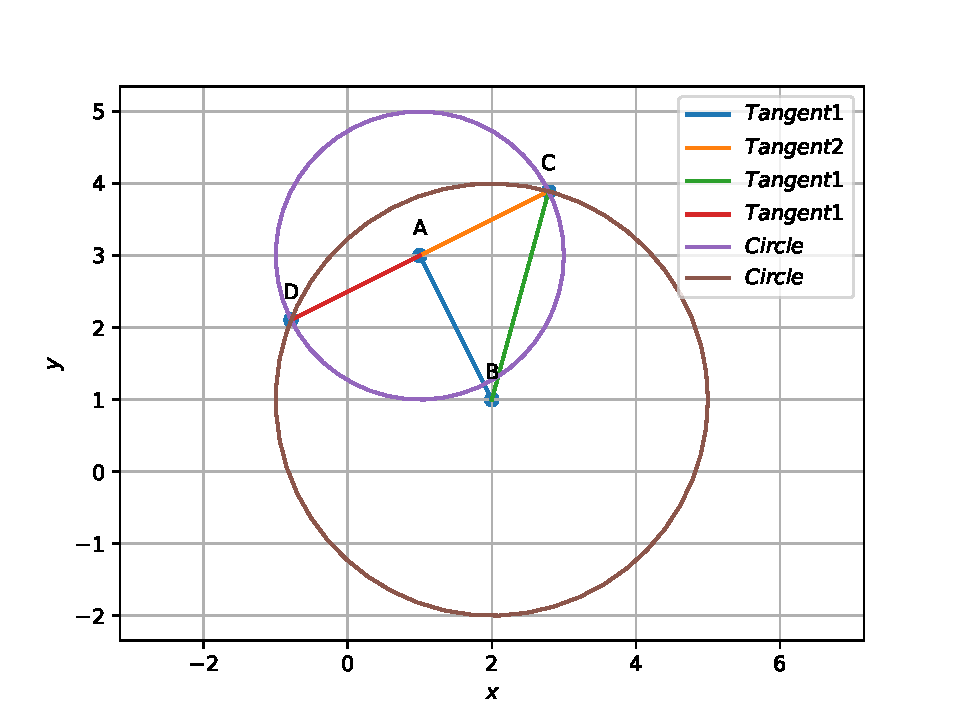
\includegraphics[scale=0.49]{figs13.pdf}
 
 \end{center}
  
    The input parameters for this construction are 
\begin{center}
\begin{tabular}{|c|c|c|}
	\hline
	\textbf{Symbol}&\textbf{Value}&\textbf{Description}\\

	\hline
		$\vec{B}$&\myvec{2\\1}&centre of circle 2\\[8pt]
	\hline
	\end{tabular}
\end{center}
\section*{Solution}
   \textbf{Statement:}
The equation of  a conic is given by 
\begin{align}
    \vec{x}^{\top}\vec{V}\vec{x}+2\vec{u}^{\top}\vec{x}+f=0
    \end{align}
 

		   
		\textbf{} From the given information,

		    \begin{align}
		        x^2 +y^2-2x-6y+6 &= 0
         \end{align}
         
 The circle can be expressed as conics,
 \\
 \begin{align}
      \vec{V} = I 
 \end{align}
   \begin{align}
\vec{u} = \myvec{-1 \\ -3}  
   \end{align}
   \\
   \begin{align}
       f=6
   \end{align}
   \\
   \begin{align}
        \vec{A} &= - \vec{V}^{-1}\vec{u}
         = \myvec{1 \\ 3}
   \end{align}
    \textbf{} equation of diameter
         \begin{align}
           \vec{n}^{\top} (\vec{X}-\vec{A})=0
           \\
           \vec{n}=\vec{A}-\vec{B}
         \end{align}
 Thus, the desired solution is the point of intersection of the line with the circle in the first quadrant as shown in Fig.  
	  
		    Using the parameteric equation of the line 
		 
		    \begin{multline}
    			   \brak{ \vec{A_1} + \lambda \vec{m}}^{\top}
			    \brak{ \vec{A_1} + \lambda \vec{m}}
			    = r^2
			    \\
			    \implies \lambda^2\norm{\vec{m}}^2+ 2 \lambda \vec{m}^{\top}\vec{A_1}
			    +\norm{\vec{A_1}}^2 - r^2 = 0
		    \end{multline}
		  
		    \begin{align}
		\lambda = \frac{-\vec{m}^{\top}\vec{A_1}\pm \sqrt{\brak{\vec{m}^{\top}\vec{A_1}}^2 -\norm{\vec{m}}^2\brak{\norm{\vec{A_1}}^2 - r^2 }}}{\norm{\vec{m}}^2}
		    \end{align}
	
		   \begin{align}
		        \vec{n} = \myvec{1 \\ -2}, c = -5,
		        \\
	        	\vec{m} = \myvec{-2\\ -1}, 
			    \\
			    \vec{A_1} = \myvec{-5 \\ 0},  r^2 = 4
		   \end{align}
\textbf{} By substituting the values in above ,we get		   
		     \begin{align}
			    \lambda_1 =- 2.1
		    \end{align}
		    \\
		     \begin{align}
			    \lambda_2 = -3.9
		    \end{align}
		    \\
		    \begin{align}
			    \vec{C} = \myvec{-5 \\ 0} - 3.8 \myvec{ -2\\ -1}
			    \\
			    = \myvec{2.7 \\3.8 }
		    \end{align}
		    \begin{align}
			    \vec{D} = \myvec{-5 \\ 0} -  2.1 \myvec{-2 \\ -1}
			    \\
			    = \myvec{-0.7 \\ 2.1}
		    \end{align}
		    Thus, the points of intersection are $C$ and $D$.
		    \\
		\textbf{} The distance between the vectors 
		\begin{align}
		  \vec{C}=\myvec{2.7 \\3.8 } ,    \vec{B}=\myvec{2\\1}  
		\end{align}
    \textbf{}Using the definition   of the norm, 
		\begin{align}
\norm{\vec{C}-\vec{B}} = 3
\end{align}
 	\textbf{}  	By substituting the values of C and B in the above equation . The distance between the point C and B will be the radius of circle2 i.e 3.
 \end{document}